\section{Resultados}

A partir dos testes realizados sob orientação do planejamento, anteriormente mencionado na seção X, foram coletados os resultados do tempo de vôo do helicóptero. As amostras dos testes coletados, como pode ser visto na tabela \ref{tab:amostras}, possui os seguintes parâmetros: \textbf{clipe} que pode ser com ou sem; \textbf{AT} que representa o adesivo no topo do helicóptero, sendo com ou sem; \textbf{ADLat} é o adesivo lateral, podendo ser colocado o adesivo do lado direito ou do lado esquerdo; \textbf{AL} é a altura de partida do helicóptero, em que foi definido como 1,30 m e 2,10 m e o tempo de queda em segundos. Dessa forma, com base nestes valores de tempo, a partir das disposições dos demais parâmetros, foi feito o teste de regressão para analisar a influência da relação entre os parâmetros com o tempo.

\begin{table}[ht]
    \centering
    \caption{Resultados das amostras coletadas.}
    \begin{tabular}{rllllr}
      \hline
     & clip & AT & ADLat & AL & tempo \\ 
      \hline
    1 & S & S & E & 1.30 & 0.92 \\ 
      2 & C & S & E & 1.30 & 0.88 \\ 
      3 & S & C & E & 1.30 & 1.04 \\ 
      4 & C & C & E & 1.30 & 1.10 \\ 
      5 & S & S & D & 1.30 & 1.10 \\ 
      6 & C & S & D & 1.30 & 0.99 \\ 
      7 & S & C & D & 1.30 & 1.07 \\ 
      8 & C & C & D & 1.30 & 0.92 \\ 
      9 & S & S & E & 2.10 & 1.76 \\ 
      10 & C & S & E & 2.10 & 1.23 \\ 
      11 & S & C & E & 2.10 & 1.88 \\ 
      12 & C & C & E & 2.10 & 1.52 \\ 
      13 & S & S & D & 2.10 & 1.70 \\ 
      14 & C & S & D & 2.10 & 1.72 \\ 
      15 & S & C & D & 2.10 & 1.46 \\ 
      16 & C & C & D & 2.10 & 1.42 \\ 
       \hline
    \end{tabular}
    \label{tab:amostras}
\end{table}

A análise de regressão deste sistema foi divida em 2 modelos: primeira e segunda ordem. Como o sistema possui 4 variáveis independentes, o modelo máximo atingido pode ser representado pela relação entre os 4 parâmetros. Porém, a partir do terceiro modelo não há mais significância entre os resultados obtidos, que será mostrado em diante, descartando assim a análise com um número maior de relações. 

\subsection{Análise de Primeira Ordem - Modelo 1}

A partir da análise linear aplicada aos resultados das amostras, aplicando-se a primeira ordem, o resultado é mostrado na tabela \ref{tab:model1}. O primeiro modelo dessa análise pode ser visualizado na Equação \ref{eq:model1}. Esta equação mostra um modelo que consegue explicar o valor do tempo a partir da relação entre os parâmetros. Os valores dentro dos parâmetros são as variáveis que mais apresentaram valores significantes ao sistema, dentre as opções estabelecidas. 

\begin{table}[ht]
    \centering
    \caption{Resultado da análise linear de primeira ordem do modelo 1.}
    \begin{tabular}{rrrrr}
      \hline
     & Estimate & Std. Error & t value & Pr($>$$|$t$|$) \\ 
      \hline
    (Intercept) & 1.0622 & 0.0910 & 11.67 & 1.54e-07 \\ 
      clipC & -0.1419 & 0.0814 & -1.74 & 0.1092 \\ 
      ATC & 0.0119 & 0.0814 & 0.15 & 0.8866 \\ 
      ADLatD & 0.0081 & 0.0814 & 0.10 & 0.9223 \\ 
      AL2.10 & 0.5844 & 0.0814 & 7.18 & 1.80e-05 \\ 
       \hline
    \end{tabular}
    \label{tab:model1}
\end{table}

\begin{align}
    \begin{split}
    tempo &= 1.062187 - 0.141875\text{.clip(C)} + 0.011875\text{.AT(C)} \\
    & + 0.008125\text{.ADLat(D)} + 0.584375\text{.AL2,10}
    \end{split}
    \label{eq:model1}
\end{align}

Com base na tabela\ref{tab:model1}, pode ser visto que estatisticamente os estimadores dos parâmetros clipe, AT e ADLat são iguais a zero, pois, ao se assumir o nível de significância a 5\% de probabilidade, o $\rho$ valor desses coeficientes é superior a 0,05, aceitando a hipótese nula, ou seja, as estimativas desses parâmetros são números muitos próximos de zero no qual pelo teste t afirma-se que esses valores aceitam a hipótese $H_0$. Portanto, se os parâmetros clipe, AT e ADLat são estatisticamente iguais a zero, eles não precisam estar no modelo pois não vai ter nenhuma contribuição significante no valor de tempo de queda do helicóptero. Então, o novo modelo pode ser representado na equação \ref{eq2:model1}, refazendo-se a análise linear do tempo de queda com relação apenas ao parâmetro AL. O resultado dos coeficientes pode ser visto na tabela\ref{tab:model1}. 

\begin{table}[ht]
    \centering
    \caption{Análise linear da relação do tempo com AL.}
    \begin{tabular}{rrrrr}
      \hline
     & Estimate & Std. Error & t value & Pr($>$$|$t$|$) \\ 
      \hline
    (Intercept) & 1.0012 & 0.0577 & 17.35 & 7.29e-11 \\ 
      AL2.10 & 0.5844 & 0.0816 & 7.16 & 4.84e-06 \\ 
       \hline
    \end{tabular}
    \label{tab2:model1}
\end{table}

\begin{align}
    tempo = 1.00125 + 0.58438\text{.AL2,10}
    \label{eq2:model1}
\end{align}

O modelo apresentado na equação \ref{eq:model1}, que representa uma regressão múltipla, foi reduzido para uma regressão simples, representado pela equação \ref{eq2:model1}. Desse modo, para explicar a equação reduzida pode-se dizer que para cada acréscimo a partir da altura de 2,10 m, o tempo de queda aumenta em 0,58 s. Com base no valor do $R^2$, que foi de 78,56\%, pode se afirmar a porcentagem do dados que são explicados pelo modelo da equação \ref{eq2:model1}. O valor do $R^2$ ajustado será desconsiderado pois esse último modelo foi o único em que todos os estimadores dos parâmetros foram significativos, no caso dessa análise linear do modelo 1. 

Analisando os resíduos do modelo 1 simplificado, foi aplicado o teste de normalidade de \textit{Shapiro-Wilk}. Nesse teste pode-se afirmar que, a partir da verificação dos resíduos desse modelo mostrou-se que no teste da normalidade apresentou um valor de 0,97528 com o $\rho$ valor respectivo de 0,9152, e adotando o nível de significância de 5\%, não houve violação da normalidade dos resíduos. Então, pode-se concluir que esses erros (resíduos) tem uma distribuição normal, como pode ser visto nos gráficos das figuras \ref{fig:qq} e \ref{fig:hist}. Dessa forma, assume-se a independência dos resíduos pelo fato que a estrutura de coleta declara essa independência. Portanto, não é preciso atribuir testes de independência.

\begin{figure}
    \centering
    \caption{Distribuição normal dos resíduos.}
    % Created by tikzDevice version 0.12.3 on 2020-09-22 19:17:36
% !TEX encoding = UTF-8 Unicode
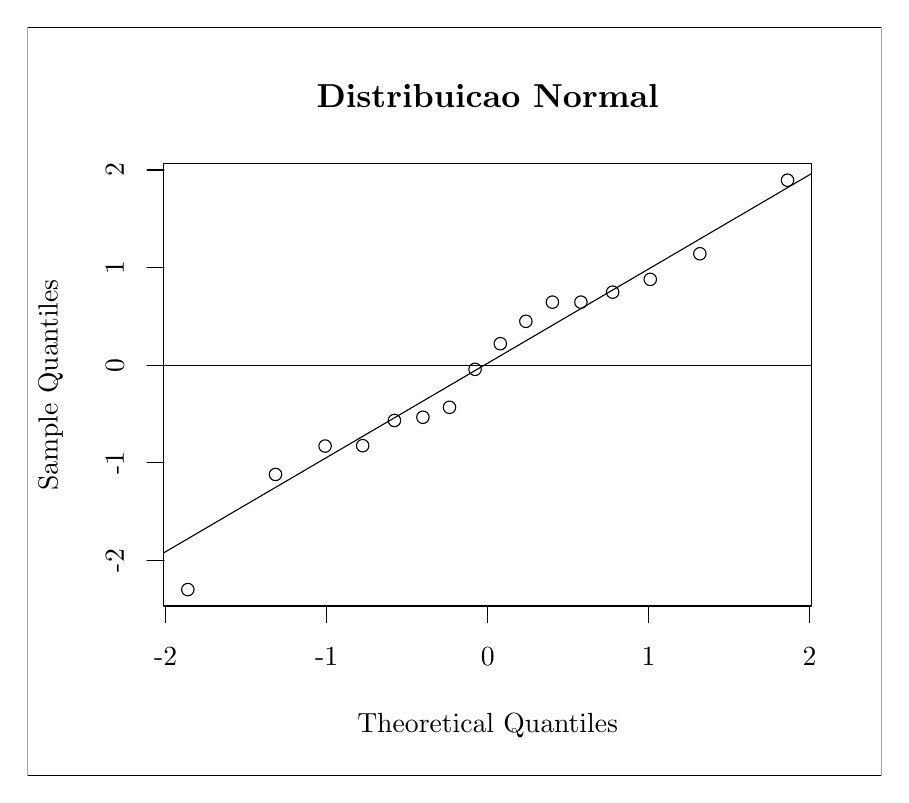
\begin{tikzpicture}[x=1pt,y=1pt]
\definecolor{fillColor}{RGB}{255,255,255}
\path[use as bounding box,fill=fillColor,fill opacity=0.00] (0,0) rectangle (308.44,270.16);
\begin{scope}
\path[clip] ( 49.20, 61.20) rectangle (283.24,220.96);
\definecolor{drawColor}{RGB}{0,0,0}

\path[draw=drawColor,line width= 0.4pt,line join=round,line cap=round] (132.53,128.22) circle (  2.25);

\path[draw=drawColor,line width= 0.4pt,line join=round,line cap=round] (107.47,118.98) circle (  2.25);

\path[draw=drawColor,line width= 0.4pt,line join=round,line cap=round] (170.78,155.96) circle (  2.25);

\path[draw=drawColor,line width= 0.4pt,line join=round,line cap=round] (189.62,170.98) circle (  2.25);

\path[draw=drawColor,line width= 0.4pt,line join=round,line cap=round] (199.91,170.98) circle (  2.25);

\path[draw=drawColor,line width= 0.4pt,line join=round,line cap=round] (161.66,146.71) circle (  2.25);

\path[draw=drawColor,line width= 0.4pt,line join=round,line cap=round] (180.02,164.05) circle (  2.25);

\path[draw=drawColor,line width= 0.4pt,line join=round,line cap=round] (142.82,129.38) circle (  2.25);

\path[draw=drawColor,line width= 0.4pt,line join=round,line cap=round] (242.89,188.46) circle (  2.25);

\path[draw=drawColor,line width= 0.4pt,line join=round,line cap=round] ( 57.87, 67.12) circle (  2.25);

\path[draw=drawColor,line width= 0.4pt,line join=round,line cap=round] (274.57,215.04) circle (  2.25);

\path[draw=drawColor,line width= 0.4pt,line join=round,line cap=round] (152.42,132.99) circle (  2.25);

\path[draw=drawColor,line width= 0.4pt,line join=round,line cap=round] (211.38,174.59) circle (  2.25);

\path[draw=drawColor,line width= 0.4pt,line join=round,line cap=round] (224.97,179.21) circle (  2.25);

\path[draw=drawColor,line width= 0.4pt,line join=round,line cap=round] (121.06,119.12) circle (  2.25);

\path[draw=drawColor,line width= 0.4pt,line join=round,line cap=round] ( 89.55,108.72) circle (  2.25);
\end{scope}
\begin{scope}
\path[clip] (  0.00,  0.00) rectangle (308.44,270.16);
\definecolor{drawColor}{RGB}{0,0,0}

\path[draw=drawColor,line width= 0.4pt,line join=round,line cap=round] ( 49.88, 61.20) -- (282.56, 61.20);

\path[draw=drawColor,line width= 0.4pt,line join=round,line cap=round] ( 49.88, 61.20) -- ( 49.88, 55.20);

\path[draw=drawColor,line width= 0.4pt,line join=round,line cap=round] (108.05, 61.20) -- (108.05, 55.20);

\path[draw=drawColor,line width= 0.4pt,line join=round,line cap=round] (166.22, 61.20) -- (166.22, 55.20);

\path[draw=drawColor,line width= 0.4pt,line join=round,line cap=round] (224.39, 61.20) -- (224.39, 55.20);

\path[draw=drawColor,line width= 0.4pt,line join=round,line cap=round] (282.56, 61.20) -- (282.56, 55.20);

\node[text=drawColor,anchor=base,inner sep=0pt, outer sep=0pt, scale=  1.00] at ( 49.88, 39.60) {-2};

\node[text=drawColor,anchor=base,inner sep=0pt, outer sep=0pt, scale=  1.00] at (108.05, 39.60) {-1};

\node[text=drawColor,anchor=base,inner sep=0pt, outer sep=0pt, scale=  1.00] at (166.22, 39.60) {0};

\node[text=drawColor,anchor=base,inner sep=0pt, outer sep=0pt, scale=  1.00] at (224.39, 39.60) {1};

\node[text=drawColor,anchor=base,inner sep=0pt, outer sep=0pt, scale=  1.00] at (282.56, 39.60) {2};

\path[draw=drawColor,line width= 0.4pt,line join=round,line cap=round] ( 49.20, 77.59) -- ( 49.20,218.72);

\path[draw=drawColor,line width= 0.4pt,line join=round,line cap=round] ( 49.20, 77.59) -- ( 43.20, 77.59);

\path[draw=drawColor,line width= 0.4pt,line join=round,line cap=round] ( 49.20,112.88) -- ( 43.20,112.88);

\path[draw=drawColor,line width= 0.4pt,line join=round,line cap=round] ( 49.20,148.16) -- ( 43.20,148.16);

\path[draw=drawColor,line width= 0.4pt,line join=round,line cap=round] ( 49.20,183.44) -- ( 43.20,183.44);

\path[draw=drawColor,line width= 0.4pt,line join=round,line cap=round] ( 49.20,218.72) -- ( 43.20,218.72);

\node[text=drawColor,rotate= 90.00,anchor=base,inner sep=0pt, outer sep=0pt, scale=  1.00] at ( 34.80, 77.59) {-2};

\node[text=drawColor,rotate= 90.00,anchor=base,inner sep=0pt, outer sep=0pt, scale=  1.00] at ( 34.80,112.88) {-1};

\node[text=drawColor,rotate= 90.00,anchor=base,inner sep=0pt, outer sep=0pt, scale=  1.00] at ( 34.80,148.16) {0};

\node[text=drawColor,rotate= 90.00,anchor=base,inner sep=0pt, outer sep=0pt, scale=  1.00] at ( 34.80,183.44) {1};

\node[text=drawColor,rotate= 90.00,anchor=base,inner sep=0pt, outer sep=0pt, scale=  1.00] at ( 34.80,218.72) {2};

\path[draw=drawColor,line width= 0.4pt,line join=round,line cap=round] ( 49.20, 61.20) --
	(283.24, 61.20) --
	(283.24,220.96) --
	( 49.20,220.96) --
	( 49.20, 61.20);
\end{scope}
\begin{scope}
\path[clip] (  0.00,  0.00) rectangle (308.44,270.16);
\definecolor{drawColor}{RGB}{0,0,0}

\node[text=drawColor,anchor=base,inner sep=0pt, outer sep=0pt, scale=  1.20] at (166.22,241.42) {\bfseries Distribuicao Normal};

\node[text=drawColor,anchor=base,inner sep=0pt, outer sep=0pt, scale=  1.00] at (166.22, 15.60) {Theoretical Quantiles};

\node[text=drawColor,rotate= 90.00,anchor=base,inner sep=0pt, outer sep=0pt, scale=  1.00] at ( 10.80,141.08) {Sample Quantiles};
\end{scope}
\begin{scope}
\path[clip] ( 49.20, 61.20) rectangle (283.24,220.96);
\definecolor{drawColor}{RGB}{0,0,0}

\path[draw=drawColor,line width= 0.4pt,line join=round,line cap=round] ( 49.20, 80.41) -- (283.24,217.42);
\end{scope}
\begin{scope}
\path[clip] (  0.00,  0.00) rectangle (308.44,270.16);
\definecolor{drawColor}{RGB}{0,0,0}

\path[draw=drawColor,line width= 0.4pt,line join=round,line cap=round] ( 49.88, 61.20) -- (282.56, 61.20);

\path[draw=drawColor,line width= 0.4pt,line join=round,line cap=round] ( 49.88, 61.20) -- ( 49.88, 55.20);

\path[draw=drawColor,line width= 0.4pt,line join=round,line cap=round] (108.05, 61.20) -- (108.05, 55.20);

\path[draw=drawColor,line width= 0.4pt,line join=round,line cap=round] (166.22, 61.20) -- (166.22, 55.20);

\path[draw=drawColor,line width= 0.4pt,line join=round,line cap=round] (224.39, 61.20) -- (224.39, 55.20);

\path[draw=drawColor,line width= 0.4pt,line join=round,line cap=round] (282.56, 61.20) -- (282.56, 55.20);

\path[draw=drawColor,line width= 0.4pt,line join=round,line cap=round] ( 49.20, 77.59) -- ( 49.20,218.72);

\path[draw=drawColor,line width= 0.4pt,line join=round,line cap=round] ( 49.20, 77.59) -- ( 43.20, 77.59);

\path[draw=drawColor,line width= 0.4pt,line join=round,line cap=round] ( 49.20,112.88) -- ( 43.20,112.88);

\path[draw=drawColor,line width= 0.4pt,line join=round,line cap=round] ( 49.20,148.16) -- ( 43.20,148.16);

\path[draw=drawColor,line width= 0.4pt,line join=round,line cap=round] ( 49.20,183.44) -- ( 43.20,183.44);

\path[draw=drawColor,line width= 0.4pt,line join=round,line cap=round] ( 49.20,218.72) -- ( 43.20,218.72);
\end{scope}
\begin{scope}
\path[clip] ( 49.20, 61.20) rectangle (283.24,220.96);
\definecolor{drawColor}{RGB}{0,0,0}

\path[draw=drawColor,line width= 0.4pt,line join=round,line cap=round] ( 49.20,148.16) -- (283.24,148.16);
\end{scope}
\begin{scope}
\path[clip] (  0.00,  0.00) rectangle (308.44,270.16);
\definecolor{drawColor}{RGB}{0,0,0}

\path[draw=drawColor,line width= 0.4pt,line join=round,line cap=round] (  0.00,  0.00) --
	(308.44,  0.00) --
	(308.44,270.16) --
	(  0.00,270.16) --
	(  0.00,  0.00);
\end{scope}
\end{tikzpicture}

    \label{fig:qq}
\end{figure}

\begin{figure}
    \centering
    \caption{Histograma dos resíduos.}
    % Created by tikzDevice version 0.12.3 on 2020-09-22 19:19:05
% !TEX encoding = UTF-8 Unicode
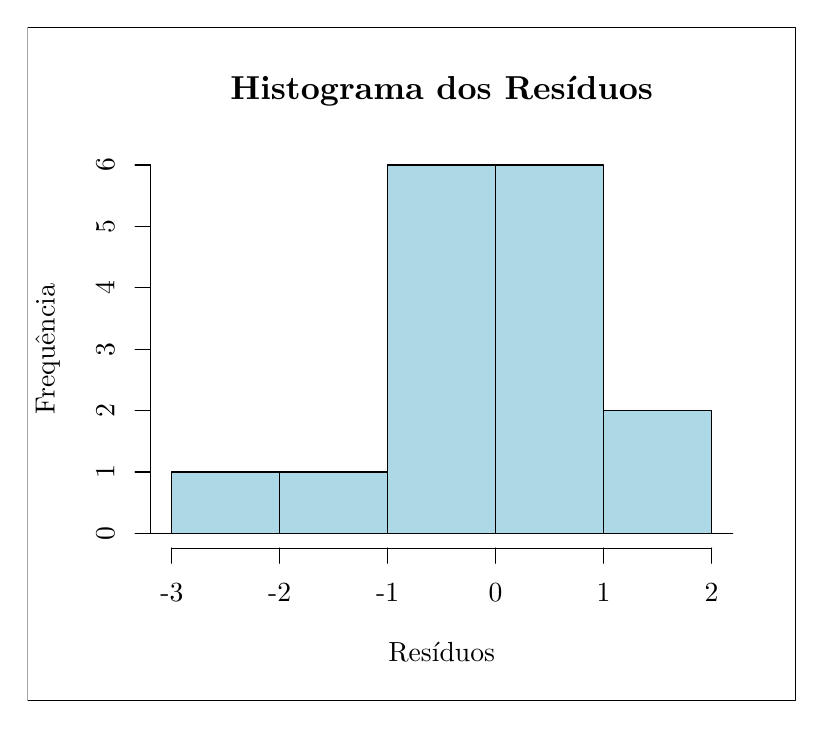
\begin{tikzpicture}[x=1pt,y=1pt, scale=0.9]
\definecolor{fillColor}{RGB}{255,255,255}
\path[use as bounding box,fill=fillColor,fill opacity=0.00] (0,0) rectangle (308.44,270.16);
\begin{scope}
\path[clip] (  0.00,  0.00) rectangle (308.44,270.16);
\definecolor{drawColor}{RGB}{0,0,0}

\node[text=drawColor,anchor=base,inner sep=0pt, outer sep=0pt, scale=  1.20] at (166.22,241.42) {\bfseries Histograma dos Resíduos};

\node[text=drawColor,anchor=base,inner sep=0pt, outer sep=0pt, scale=  1.00] at (166.22, 15.60) {Resíduos};

\node[text=drawColor,rotate= 90.00,anchor=base,inner sep=0pt, outer sep=0pt, scale=  1.00] at ( 10.80,141.08) {Frequência};
\end{scope}
\begin{scope}
\path[clip] (  0.00,  0.00) rectangle (308.44,270.16);
\definecolor{drawColor}{RGB}{0,0,0}

\path[draw=drawColor,line width= 0.4pt,line join=round,line cap=round] ( 57.87, 61.20) -- (274.57, 61.20);

\path[draw=drawColor,line width= 0.4pt,line join=round,line cap=round] ( 57.87, 61.20) -- ( 57.87, 55.20);

\path[draw=drawColor,line width= 0.4pt,line join=round,line cap=round] (101.21, 61.20) -- (101.21, 55.20);

\path[draw=drawColor,line width= 0.4pt,line join=round,line cap=round] (144.55, 61.20) -- (144.55, 55.20);

\path[draw=drawColor,line width= 0.4pt,line join=round,line cap=round] (187.89, 61.20) -- (187.89, 55.20);

\path[draw=drawColor,line width= 0.4pt,line join=round,line cap=round] (231.23, 61.20) -- (231.23, 55.20);

\path[draw=drawColor,line width= 0.4pt,line join=round,line cap=round] (274.57, 61.20) -- (274.57, 55.20);

\node[text=drawColor,anchor=base,inner sep=0pt, outer sep=0pt, scale=  1.00] at ( 57.87, 39.60) {-3};

\node[text=drawColor,anchor=base,inner sep=0pt, outer sep=0pt, scale=  1.00] at (101.21, 39.60) {-2};

\node[text=drawColor,anchor=base,inner sep=0pt, outer sep=0pt, scale=  1.00] at (144.55, 39.60) {-1};

\node[text=drawColor,anchor=base,inner sep=0pt, outer sep=0pt, scale=  1.00] at (187.89, 39.60) {0};

\node[text=drawColor,anchor=base,inner sep=0pt, outer sep=0pt, scale=  1.00] at (231.23, 39.60) {1};

\node[text=drawColor,anchor=base,inner sep=0pt, outer sep=0pt, scale=  1.00] at (274.57, 39.60) {2};

\path[draw=drawColor,line width= 0.4pt,line join=round,line cap=round] ( 49.20, 67.12) -- ( 49.20,215.04);

\path[draw=drawColor,line width= 0.4pt,line join=round,line cap=round] ( 49.20, 67.12) -- ( 43.20, 67.12);

\path[draw=drawColor,line width= 0.4pt,line join=round,line cap=round] ( 49.20, 91.77) -- ( 43.20, 91.77);

\path[draw=drawColor,line width= 0.4pt,line join=round,line cap=round] ( 49.20,116.42) -- ( 43.20,116.42);

\path[draw=drawColor,line width= 0.4pt,line join=round,line cap=round] ( 49.20,141.08) -- ( 43.20,141.08);

\path[draw=drawColor,line width= 0.4pt,line join=round,line cap=round] ( 49.20,165.73) -- ( 43.20,165.73);

\path[draw=drawColor,line width= 0.4pt,line join=round,line cap=round] ( 49.20,190.39) -- ( 43.20,190.39);

\path[draw=drawColor,line width= 0.4pt,line join=round,line cap=round] ( 49.20,215.04) -- ( 43.20,215.04);

\node[text=drawColor,rotate= 90.00,anchor=base,inner sep=0pt, outer sep=0pt, scale=  1.00] at ( 34.80, 67.12) {0};

\node[text=drawColor,rotate= 90.00,anchor=base,inner sep=0pt, outer sep=0pt, scale=  1.00] at ( 34.80, 91.77) {1};

\node[text=drawColor,rotate= 90.00,anchor=base,inner sep=0pt, outer sep=0pt, scale=  1.00] at ( 34.80,116.42) {2};

\node[text=drawColor,rotate= 90.00,anchor=base,inner sep=0pt, outer sep=0pt, scale=  1.00] at ( 34.80,141.08) {3};

\node[text=drawColor,rotate= 90.00,anchor=base,inner sep=0pt, outer sep=0pt, scale=  1.00] at ( 34.80,165.73) {4};

\node[text=drawColor,rotate= 90.00,anchor=base,inner sep=0pt, outer sep=0pt, scale=  1.00] at ( 34.80,190.39) {5};

\node[text=drawColor,rotate= 90.00,anchor=base,inner sep=0pt, outer sep=0pt, scale=  1.00] at ( 34.80,215.04) {6};
\end{scope}
\begin{scope}
\path[clip] ( 49.20, 61.20) rectangle (283.24,220.96);
\definecolor{drawColor}{RGB}{0,0,0}
\definecolor{fillColor}{RGB}{173,216,230}

\path[draw=drawColor,line width= 0.4pt,line join=round,line cap=round,fill=fillColor] ( 57.87, 67.12) rectangle (101.21, 91.77);

\path[draw=drawColor,line width= 0.4pt,line join=round,line cap=round,fill=fillColor] (101.21, 67.12) rectangle (144.55, 91.77);

\path[draw=drawColor,line width= 0.4pt,line join=round,line cap=round,fill=fillColor] (144.55, 67.12) rectangle (187.89,215.04);

\path[draw=drawColor,line width= 0.4pt,line join=round,line cap=round,fill=fillColor] (187.89, 67.12) rectangle (231.23,215.04);

\path[draw=drawColor,line width= 0.4pt,line join=round,line cap=round,fill=fillColor] (231.23, 67.12) rectangle (274.57,116.42);
\end{scope}
\begin{scope}
\path[clip] (  0.00,  0.00) rectangle (308.44,270.16);
\definecolor{drawColor}{RGB}{0,0,0}

\path[draw=drawColor,line width= 0.4pt,line join=round,line cap=round] ( 57.87, 61.20) -- (274.57, 61.20);

\path[draw=drawColor,line width= 0.4pt,line join=round,line cap=round] ( 57.87, 61.20) -- ( 57.87, 55.20);

\path[draw=drawColor,line width= 0.4pt,line join=round,line cap=round] (101.21, 61.20) -- (101.21, 55.20);

\path[draw=drawColor,line width= 0.4pt,line join=round,line cap=round] (144.55, 61.20) -- (144.55, 55.20);

\path[draw=drawColor,line width= 0.4pt,line join=round,line cap=round] (187.89, 61.20) -- (187.89, 55.20);

\path[draw=drawColor,line width= 0.4pt,line join=round,line cap=round] (231.23, 61.20) -- (231.23, 55.20);

\path[draw=drawColor,line width= 0.4pt,line join=round,line cap=round] (274.57, 61.20) -- (274.57, 55.20);

\path[draw=drawColor,line width= 0.4pt,line join=round,line cap=round] ( 49.20, 67.12) -- ( 49.20,215.04);

\path[draw=drawColor,line width= 0.4pt,line join=round,line cap=round] ( 49.20, 67.12) -- ( 43.20, 67.12);

\path[draw=drawColor,line width= 0.4pt,line join=round,line cap=round] ( 49.20, 91.77) -- ( 43.20, 91.77);

\path[draw=drawColor,line width= 0.4pt,line join=round,line cap=round] ( 49.20,116.42) -- ( 43.20,116.42);

\path[draw=drawColor,line width= 0.4pt,line join=round,line cap=round] ( 49.20,141.08) -- ( 43.20,141.08);

\path[draw=drawColor,line width= 0.4pt,line join=round,line cap=round] ( 49.20,165.73) -- ( 43.20,165.73);

\path[draw=drawColor,line width= 0.4pt,line join=round,line cap=round] ( 49.20,190.39) -- ( 43.20,190.39);

\path[draw=drawColor,line width= 0.4pt,line join=round,line cap=round] ( 49.20,215.04) -- ( 43.20,215.04);
\end{scope}
\begin{scope}
\path[clip] ( 49.20, 61.20) rectangle (283.24,220.96);
\definecolor{drawColor}{RGB}{0,0,0}

\path[draw=drawColor,line width= 0.4pt,line join=round,line cap=round] ( 49.20, 67.12) -- (283.24, 67.12);
\end{scope}
\begin{scope}
\path[clip] (  0.00,  0.00) rectangle (308.44,270.16);
\definecolor{drawColor}{RGB}{0,0,0}

\path[draw=drawColor,line width= 0.4pt,line join=round,line cap=round] (  0.00,  0.00) --
	(308.44,  0.00) --
	(308.44,270.16) --
	(  0.00,270.16) --
	(  0.00,  0.00);
\end{scope}
\end{tikzpicture}

    \label{fig:hist}
\end{figure}

\subsection{Análise de Segunda Ordem - Modelo 2}

No modelo 2 foi feito a análise linear de segunda ordem. O resultado dessa análise pode ser visto na tabela \ref{tab:model2}. A partir dos valores da tabela \ref{tab:model2} foi calculado o modelo 2, representado pela equação \ref{eq:model2}.


\begin{table}[ht]
    \centering
    \caption{Resultado da análise linear de segunda ordem.}
    \begin{tabular}{rrrrr}
      \hline
     & Estimate & Std. Error & t value & Pr($>$$|$t$|$) \\ 
      \hline
    (Intercept) & 0.9203 & 0.0206 & 44.73 & 0.0142 \\ 
      clipC & -0.0506 & 0.0281 & -1.80 & 0.3227 \\ 
      ATC & 0.1094 & 0.0281 & 3.89 & 0.1602 \\ 
      ADLatD & 0.1744 & 0.0281 & 6.20 & 0.1018 \\ 
      AL2.10 & 0.8344 & 0.0281 & 29.68 & 0.0214 \\ 
      clipC:ATC & 0.1262 & 0.0368 & 3.43 & 0.1806 \\ 
      clipC:ADLatD & -0.0438 & 0.0368 & -1.19 & 0.4453 \\ 
      clipC:AL2.10 & -0.4638 & 0.0368 & -12.60 & 0.0504 \\ 
      ATC:ADLatD & -0.1288 & 0.0368 & -3.50 & 0.1773 \\ 
      ATC:AL2.10 & 0.0162 & 0.0368 & 0.44 & 0.7353 \\ 
      ADLatD:AL2.10 & -0.2238 & 0.0368 & -6.08 & 0.1038 \\ 
      clipC:ATC:ADLatD & -0.1925 & 0.0425 & -4.53 & 0.1383 \\ 
      clipC:ATC:AL2.10 & 0.0225 & 0.0425 & 0.53 & 0.6900 \\ 
      clipC:ADLatD:AL2.10 & 0.5675 & 0.0425 & 13.35 & 0.0476 \\ 
      ATC:ADLatD:AL2.10 & -0.2475 & 0.0425 & -5.82 & 0.1083 \\ 
       \hline
    \end{tabular}
    \label{tab:model2}
\end{table}

\begin{align}
    \begin{split}
    tempo &= 0.93906 - 0.15\text{.clipC} + 0.21375\text{.ATC} + 0.1425\text{.ADLatD}  \\
    & + 0.74875\text{.AL2,10} + 0.04125\text{.clipC.ATC} + 0.14375\text{.clipC.ADLatD} \\
    & - 0.16875\text{.clipC.AL2,10} - 0.34875\text{.ATC.ADLatD} - 0.09625\text{.ATC.AL2,10} \\
    & - 0.06375\text{.ADLatD.AL2,10}
    \end{split}
\label{eq:model2}
\end{align}

Essa equação do modelo 2 consegue explicar o valor do tempo a partir da relação de segunda ordem dos parâmetros. Como pode ser visto na tabela \ref{tab:model2}, o parâmetro que possui os estimadores mais significantes, se assumir o nível de significância de 5\%, é novamente o AL, ou seja, estatisticamente os valores do $\rho$ valor são maiores que 0.05 em todos exceto o AL2,10. Como isso considera a hipótese nula em que as estimativas desses coeficientes possuem valores muito próximo de zero, podendo também ser retirado da equação da relação de segunda ordem, pois, estatisticamente esses parâmetros não apresentam contribuição significativa no valor do tempo de queda do helicóptero. Desta maneira, simplificando a equação \ref{eq:model2} do modelo 2 irá ficar da mesma forma que a equação \ref{eq2:model1}, propiciando o encerramento da análise de regressão para o modelo 2.
 
